\begin{center}
    \textbf{BAB III} \\[0.5em]
    \textbf{METODE PENELITIAN}
\end{center}

\subsection*{3.1 Pengertian Metodologi Penulisan}
\textbf{Pengertian Metodologi Penulisan}

Metodologi penulisan merupakan bagian dari ilmu pengetahuan yang mempelajari bagaimana prosedur kerja mencari kebenaran (Muhajir, 2000). Metodologi adalah awal dari metode dan lebih mendasar dibandingkan metode. Metodologi menyediakan dasar-dasar kerja filosofis bagi sebuah metode (Kuswarno, 2009).

Metode penulisan mengacu pada prosedur tertentu untuk mengumpulkan dan menganalisis data (Wilis, 2007). Metode untuk penulisan kuantitatif berbeda dengan penulisan kualitatif. Penulisan kualitatif adalah jenis penulisan yang menghasilkan penemuan-penemuan yang tidak dapat diperoleh dengan menggunakan prosedur statistik atau cara-cara lain dari kuantifikasi (Creswell, 2007). Metode penulisan merupakan cara ilmiah untuk mendapatkan data dengan tujuan dan kegunaan tertentu (Sugiyono, 2017, 3). Cara ilmiah berarti penulisan didasarkan pada ciri-ciri keilmuan yaitu:
\begin{itemize}
    \item Rasional, artinya penulisan dilakukan dengan cara yang masuk akal.
    \item Empiris, artinya cara-cara yang digunakan dapat diamati.
    \item Sistematis, artinya penulisan menggunakan langkah-langkah tertentu yang bersifat logis.
\end{itemize}

\subsection*{3.2 Metodologi Pengembangan Sistem}
Metodologi yang digunakan dalam pengembangan sistem aplikasi \textit{task tracker} berbasis web ini adalah \textit{Agile Methodology}. \textit{Agile} merupakan pendekatan pengembangan perangkat lunak yang bersifat iteratif dan inkremental, serta menekankan kolaborasi, fleksibilitas, dan adaptasi terhadap perubahan kebutuhan pengguna.

Metodologi ini terdiri atas beberapa tahapan:
\begin{enumerate}
    \item \textbf{Requirement Gathering} (Pengumpulan Kebutuhan)
    \newline Pada tahap ini dilakukan identifikasi kebutuhan sistem aplikasi \textit{task tracker} berdasarkan permasalahan yang ingin diselesaikan, yaitu manusia sering kali dihadapkan pada berbagai aktivitas dan tanggung jawab yang harus diselesaikan dalam waktu tertentu. 
    Namun, tidak jarang kita lupa apa yang sudah dikerjakan sebelumnya, atau bingung menentukan apa yang harus dilakukan selanjutnya. 
    Hal ini bisa menyebabkan penurunan produktivitas, ketidakteraturan, dan bahkan stres akibat pekerjaan yang menumpuk tanpa perencanaan.
    \newline Untuk mengatasi permasalahan tersebut, dibutuhkan sebuah sistem yang dapat membantu individu dalam mencatat, mengelola, dan melacak kegiatan sehari-hari secara terstruktur.
    Aplikasi \textit{task tracker} hadir sebagai solusi praktis untuk mencatat aktivitas harian, mengingatkan tugas yang belum selesai, dan memberikan gambaran yang jelas mengenai progres harian maupun mingguan pengguna.
    \item \textbf{Design} (Perancangan)
    Desain dilakukan secara bertahap dan langsung mendukung fitur yang akan dikembangkan. Karena pengerjaan dilakukan secara mandiri dan tidak formal, desain difokuskan pada: Struktur basis data menggunakan PostgreSQL. Arsitektur MVC dengan Laravel (PHP webframework). 
    Desain antarmuka yang sederhana dan fungsional, berfokus pada penggunaan harian.
    \item \textbf{Development} (Pengembangan/Koding)
    Setelah Pada tahap ini dilakukan implementasi kode sesuai dengan fitur yang direncanakan.
    Proses pengembangan dilakukan secara iteratif, satu fitur pada satu waktu, seperti:
    \begin{itemize}
        \item Pengerjaan fitur login dan registrasi
        \item Pengerjaan fitur workspace management
        \item Pengerjaan fitur task management
    \end{itemize}
    \item \textbf{Testing} (Pengujian)
    Pada tahap ini Setelah fitur dikembangkan, dilakukan pengujian fungsional secara manual seperti: 
    \begin{itemize}
        \item Integration Testing: Memastikan setiap bagian sistem saling terhubung dengan baik (contoh: form input tugas terhubung ke tampilan list).
        \item System Testing: Pengujian keseluruhan aplikasi melalui skenario penggunaan sehari-hari.
        \item User Acceptance Testing: Pengujian dilakukan oleh pengembang sendiri sebagai pengguna utama.
    \end{itemize}
    \item \textbf{Deployment} (Penerapan)
    Pada tahapan ini aplikasi kemudian dijalankan di lingkungan produksi lokal atau server pribadi.
    \item \textbf{Review} (Maintenance/Pemeliharaan)
    Tahap ini mencakup perbaikan bug yang ditemukan selama penggunaan, serta penambahan fitur baru berdasarkan pengalaman pribadi.
    Proses review dilakukan secara berkala: Menyempurnakan tampilan antarmuka.
    Mengoptimalkan proses pengambilan data. 
    Menambahkan fitur tambahan jika perlu
\end{enumerate}


\subsection*{3.3 Tujuan Project}
\begin{itemize}
    \item Membantu pengguna mencatat dan merencanakan aktivitas harian agar tidak ada tugas yang terlewat. 
    \item Meningkatkan produktivitas dengan pengelolaan waktu dan tugas yang lebih terorganisir.
    \item Mempermudah proses tracking kegiatan harian untuk refleksi dan evaluasi diri.
    \item Membantu pengguna membangun kebiasaan yang konsisten dalam menyelesaikan tugas-tugasnya. 
    \item Memberikan antarmuka yang sederhana dan mudah digunakan, sehingga bisa digunakan oleh siapa saja dalam berbagai aktivitas sehari-hari. 
    \item Menyediakan fitur workspace agar pengguna dapat mengelola aktivitas dalam konteks kerja sama tim atau proyek tertentu.
    \item Menyediakan fitur role management agar pengguna melakukan promosi / demosi pada member dalam workspace tersebut.
\end{itemize}

\subsection*{3.4 Batasan Projek Task Tracker}
\begin{itemize}
    \item User Management \\
    fitur ini mencakup fitur registrasi dan login user, sehingga data pada website bisa terhubung sesuai dengan user yang sedang login.
    website juga mempunyai menu profile sehingga user bisa mengupdate nama user dan password jika dibutuhkan
    \item Workspace Management \\
    fitur ini berguna agar user bisa membuat workspace baru, mengedit workspace, dan menghapus workspace.
    \item Member Management \\
    fitur ini berguna agar user bisa melihat member yang ada di dalam workspace tersebut, dan member bisa melakukan management member seusai dengan role yang dimiliki.
    seperti promosi / demosi member, menghapus member, dan mengundang user lain untuk bergabung ke dalam workspace tersebut
    \item Role Management \\
    fitur ini berguna agar user melakukan manajemen role pada workspace tersebut, seperti promosi / demosi member, role di dalam workspace dibagi menjadi 3 yaitu member, admin, dan owner.
    \\ tugas dari masing-masing role adalah sebagai berikut:
    \begin{itemize}
      \item Owner: bisa melakukan manajemen task (CRUD), invite user lain ke dalam workspace, menghapus member, menghapus workspace, dan promosi / demosi member.
      owner juga bisa memindahkan privilige owner kepada admin lainnya, di case tersebut owner akan menjadi admin.
      \item Admin: bisa melakukan manajemen task (CRUD), promosi admin dan menghapus member.
      \item Member: bisa melihat dan menggeser task status.
    \end{itemize}
    \item Task Management \\
    fitur ini berguna agar user bisa membuat task baru, mengedit task, menghapus task, dan menugaskan user ke dalam task tersebut.
    \item Task Board \\
    di halaman ini user bisa melihat task dalam bentuk board, board terdiri dari 3 status yaitu todo, in progress, dan done. 
    sehingga user lebih mudah mengelola task yang ada di dalam workspace tersebut.
    \item Dashboard \\
    Fitur dashboard berguna agar user bisa melihat summary dari semua task di dalam workspace yang diikuti oleh pengguna.
\end{itemize}

\subsection*{3.5 Usecase Diagram}
\begin{itemize}
  \item User Management
  \begin{center}
    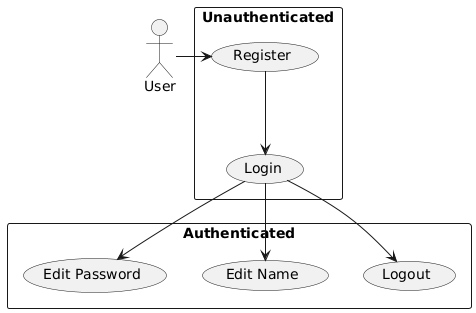
\includegraphics[width=0.5\textwidth]{assets/usecase_diagrams/auth.png}
    \captionof{figure}{Usecase Diagram User Management}
  \end{center}
  pada usecase diagram diatas ini dijelaskan bahwa user yang belum terautentikasi bisa melakukan registrasi terlebih dahulu untuk bisa menggunakan aplikasi ini.
  setelah melakukan registrasi, user bisa melakukan login untuk bisa menggunakan aplikasi ini. user juga bisa mengubah profile yang sudah dibuat (nama dan password).
  setelah login, user bisa melakukan logout untuk bisa keluar dari aplikasi ini.
  \item Workspace Management
  \begin{center}
    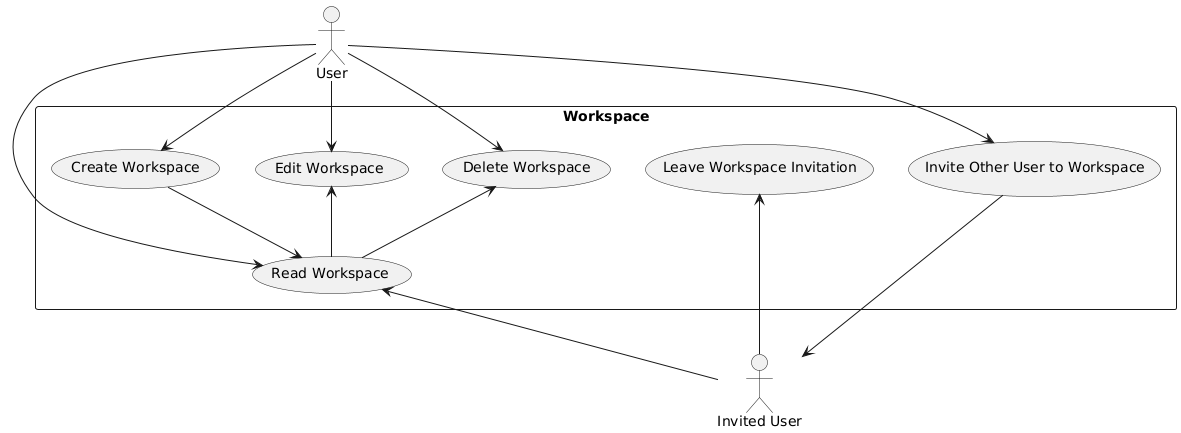
\includegraphics[width=0.8\textwidth]{assets/usecase_diagrams/workspace.png}
    \captionof{figure}{Usecase Diagram Workspace Management}
  \end{center}
  pada usecase diagram diatas ini dijelaskan bahwa user bisa membuat workspace baru, mengedit workspace, menghapus workspace, dan mengundang user lain untuk bergabung ke dalam workspace tersebut.
  \item Role Management
  \begin{center}
    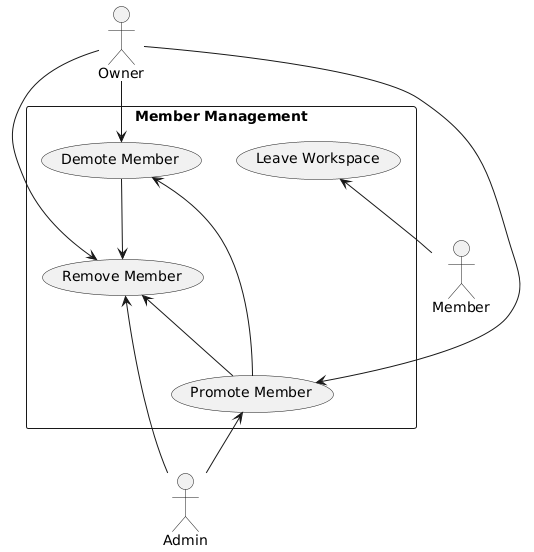
\includegraphics[width=0.5\textwidth]{assets/usecase_diagrams/role.png}
    \captionof{figure}{Usecase Diagram Role Management}
  \end{center}
  pada usecase diagram diatas ini dijelaskan bahwa user bisa melakukan manajemen role pada workspace tersebut, seperti promosi / demosi member, role di dalam workspace dibagi menjadi 3 yaitu member, admin, dan owner.
  \item Task Management
  \begin{center}
    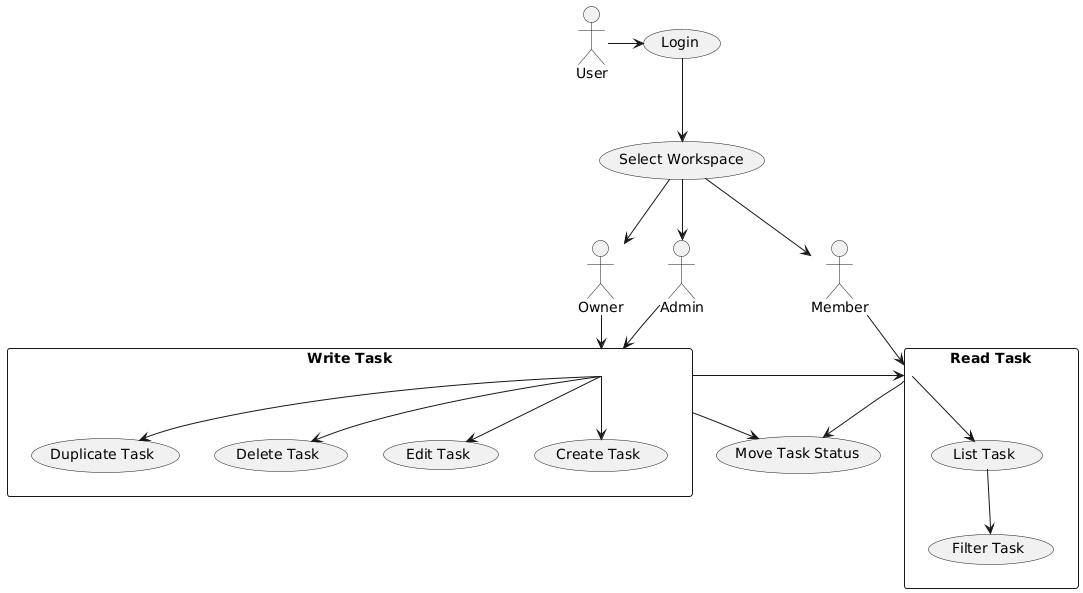
\includegraphics[width=0.8\textwidth]{assets/usecase_diagrams/task.png}
    \captionof{figure}{Usecase Diagram Task Management}
  \end{center}
  pada usecase diagram diatas ini dijelaskan bahwa untuk role admin dan owner bisa melakukan manajemen task (CRUD),
  sedangkan untuk role member bisa melihat dan menggeser task status.
\end{itemize}

\subsection*{3.6 Class Diagram}
ini adalah class diagram yang menjelaskan model data dan hubungan antar data yang ada pada sistem.
\begin{center}
  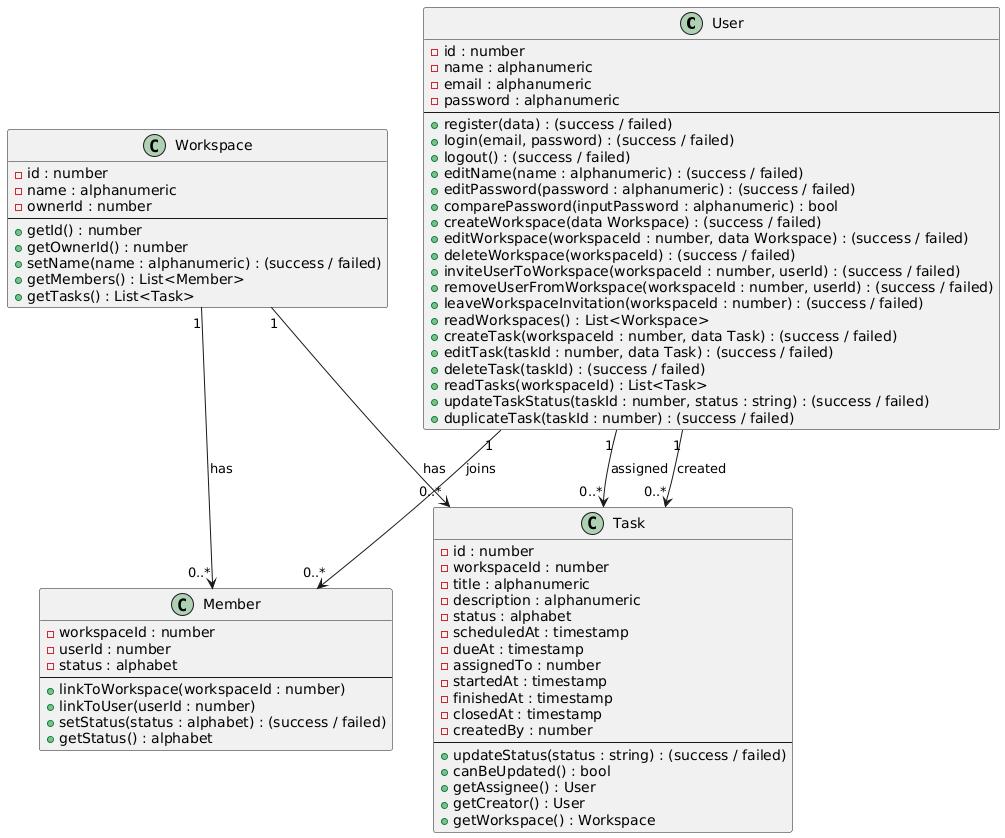
\includegraphics[width=1\textwidth]{assets/class_diagram.png}
  \captionof{figure}{Class Diagram}
\end{center}

\subsection*{3.7 Activity Diagram}

\subsubsection*{User Management}
\begin{center}
    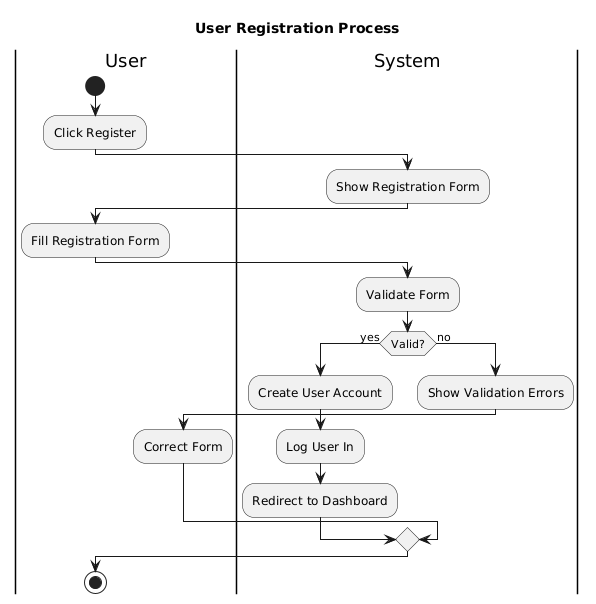
\includegraphics[width=0.5\textwidth]{assets/activity_diagrams/user_register.png}
    \captionof{figure}{Activity Diagram User Register}
\end{center}
pada activity diagram diatas menjelaskan bahwa user bisa melakukan registrasi agar bisa menggunakan aplikasi ini.

\begin{center}
    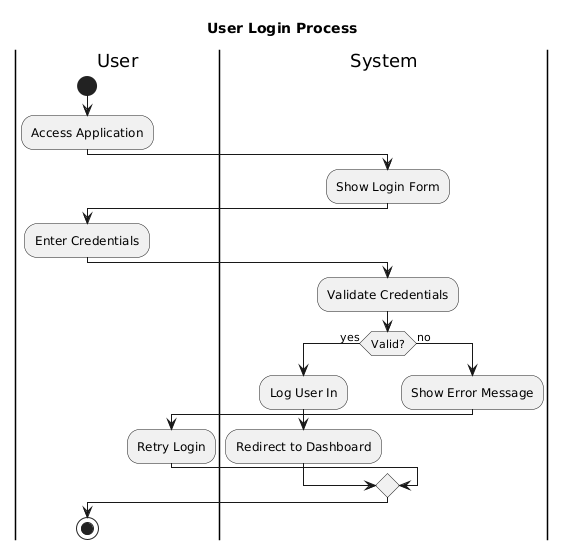
\includegraphics[width=0.5\textwidth]{assets/activity_diagrams/user_login.png}
    \captionof{figure}{Activity Diagram User Login}
\end{center}
pada activity diagram diatas menjelaskan bahwa user bisa melakukan login agar bisa mengunakan fitur-fitur yang ada pada aplikasi ini.

\begin{center}
    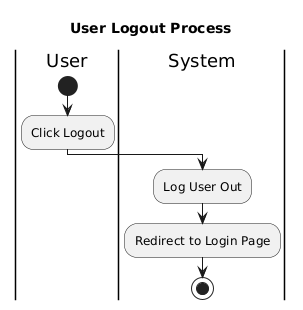
\includegraphics[width=0.5\textwidth]{assets/activity_diagrams/user_logout.png}
    \captionof{figure}{Activity Diagram User Logout}
\end{center}
pada activity diagram diatas menjelaskan bahwa setelah login, user bisa melakukan logout untuk bisa keluar dari aplikasi ini.

\begin{center}
    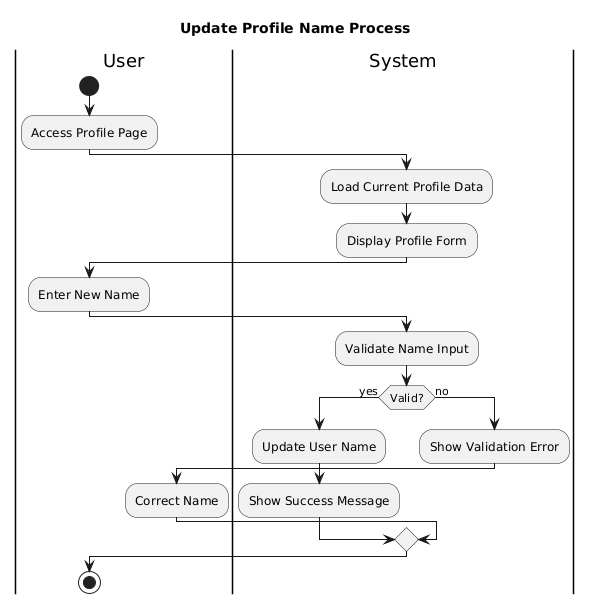
\includegraphics[width=0.5\textwidth]{assets/activity_diagrams/user_profile_update_name.png}
    \captionof{figure}{Activity Diagram User Profile Update Name}
\end{center}
pada activity diagram diatas menjelaskan bahwa user bisa mengubah nama user yang sudah dibuat.

\begin{center}
    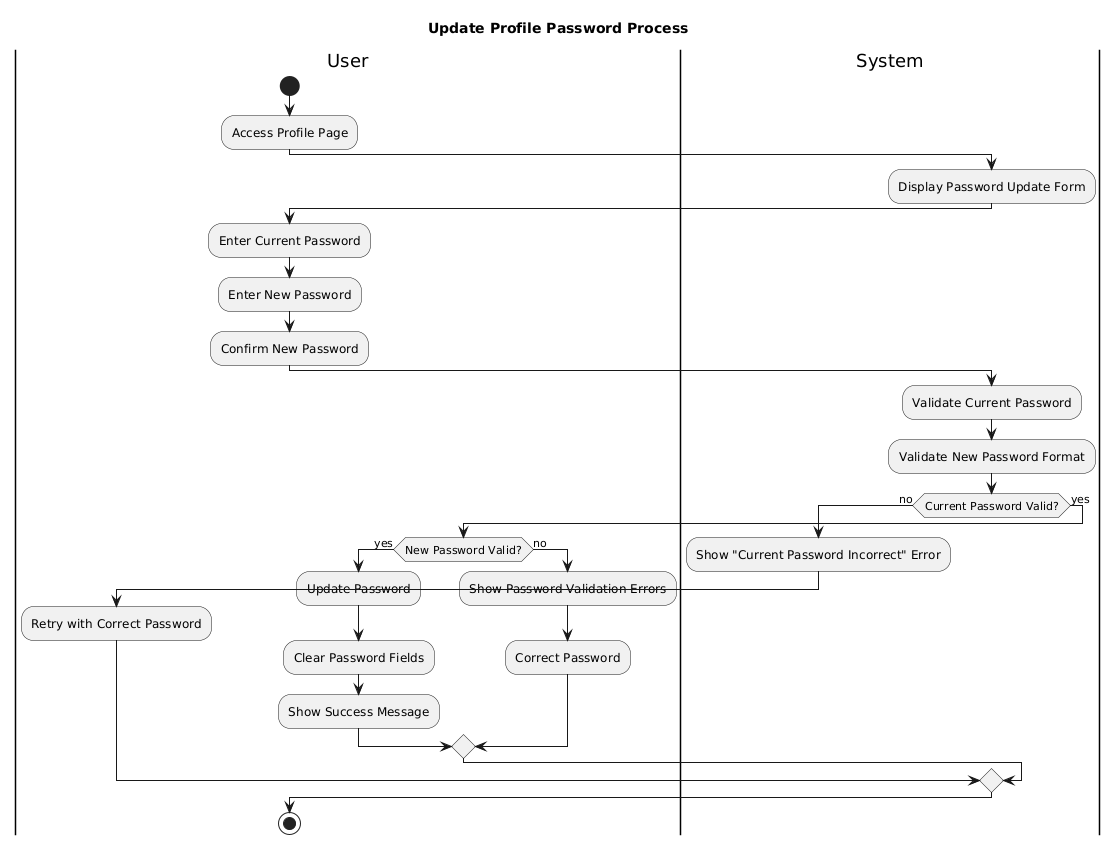
\includegraphics[width=0.5\textwidth]{assets/activity_diagrams/user_profile_update_password.png}
    \captionof{figure}{Activity Diagram User Profile Update Password}
\end{center}
pada activity diagram diatas menjelaskan bahwa user bisa mengubah password user yang sudah dibuat.

\subsubsection*{Workspace Management}
\begin{center}
    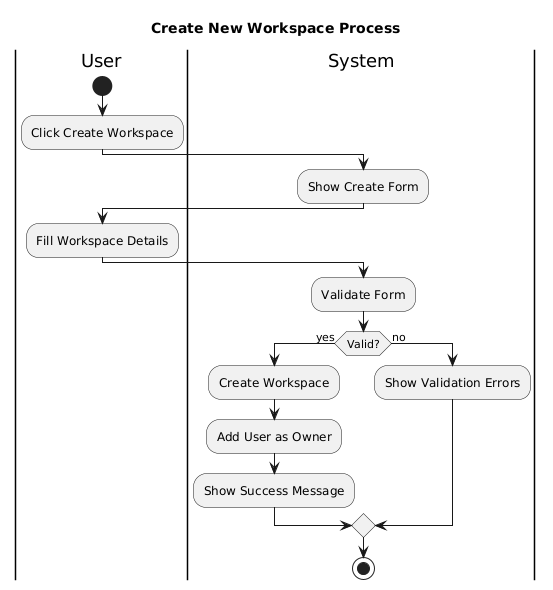
\includegraphics[width=0.5\textwidth]{assets/activity_diagrams/workspace_create.png}
    \captionof{figure}{Activity Diagram Workspace Create}
\end{center}
pada activity diagram diatas menjelaskan bahwa user bisa membuat workspace baru.
user akan menjadi owner dari workspace yang dibuat.
\begin{center}
    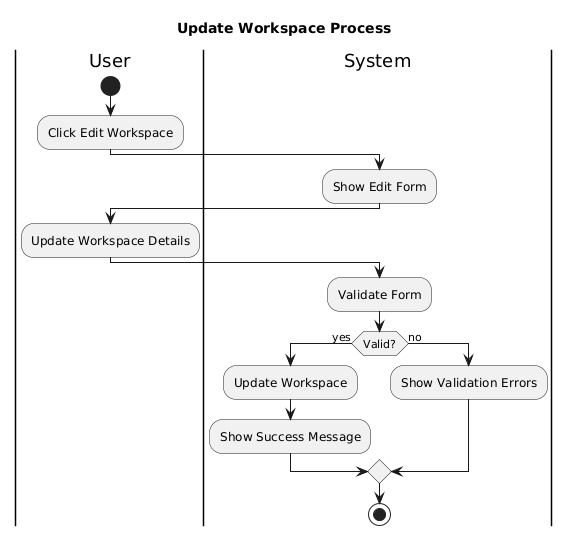
\includegraphics[width=0.5\textwidth]{assets/activity_diagrams/workspace_update.png}
    \captionof{figure}{Activity Diagram Workspace Update}
\end{center}
pada activity diagram diatas menjelaskan bahwa user bisa mengubah workspace yang sudah dibuat.
\begin{center}
    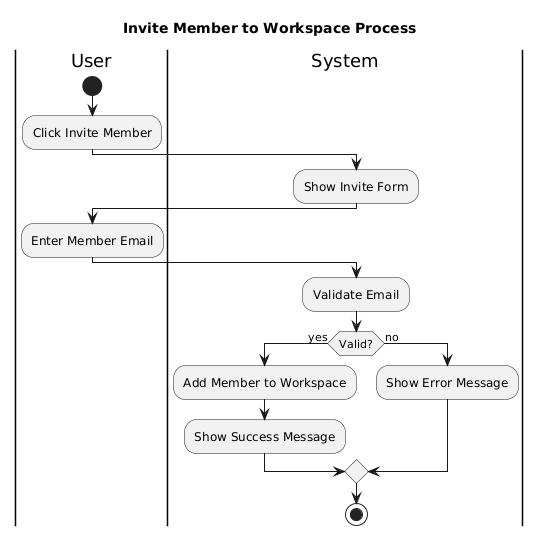
\includegraphics[width=0.5\textwidth]{assets/activity_diagrams/workspace_invite.png}
    \captionof{figure}{Activity Diagram Workspace Invite}
\end{center}
pada activity diagram diatas menjelaskan bahwa user bisa mengundang user lain untuk bergabung ke dalam workspace tersebut.
member baru otomatis memiliki role member.
\begin{center}
    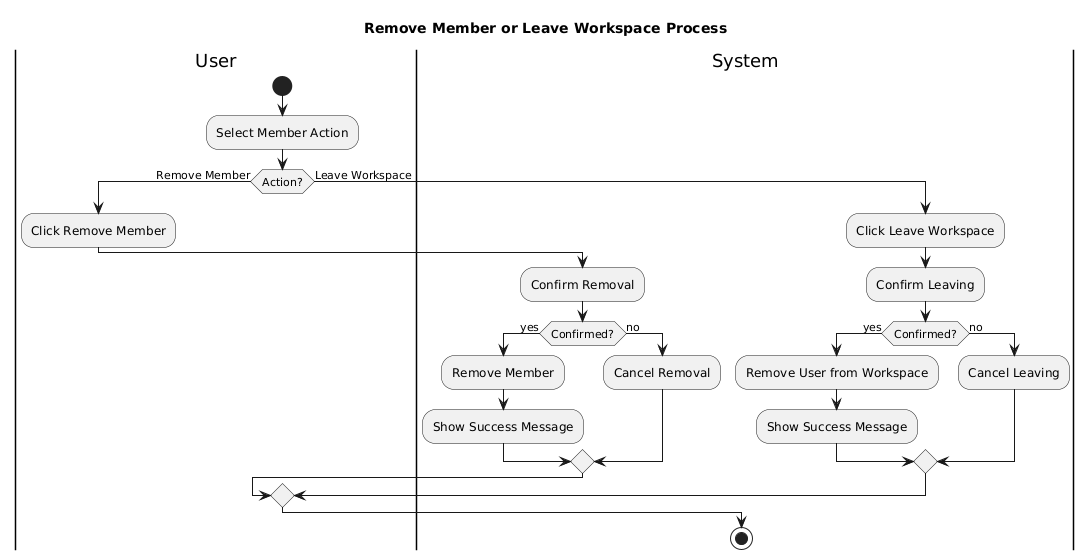
\includegraphics[width=0.8\textwidth]{assets/activity_diagrams/workspace_remove.png}
    \captionof{figure}{Activity Diagram Workspace Remove}
\end{center}
pada activity diagram diatas menjelaskan bahwa user bisa menghapus workspace yang sudah dibuat.
\begin{center}
    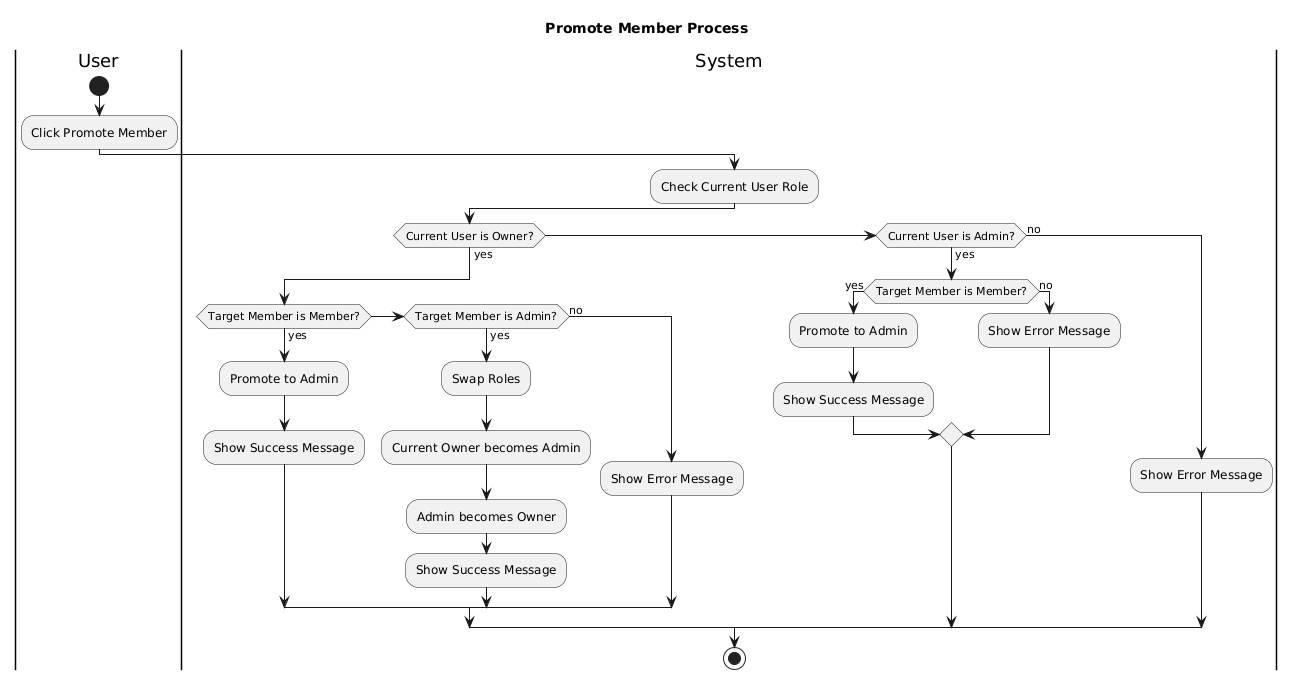
\includegraphics[width=0.8\textwidth]{assets/activity_diagrams/member_promote.png}
    \captionof{figure}{Activity Diagram Member Promote}
\end{center}
pada activity diagram diatas menjelaskan bahwa user dengan owner bisa melakukan promosi member menjadi role admin dan sebaliknya.
setelah member di promosi menjadi admin, member juga bisa di promosikan menjadi owner. sehingga owner yang lama akan menjadi admin.
sedangkan user dengan owner admin bisa melakukan promosi dari member menjadi admin.
\begin{center}
    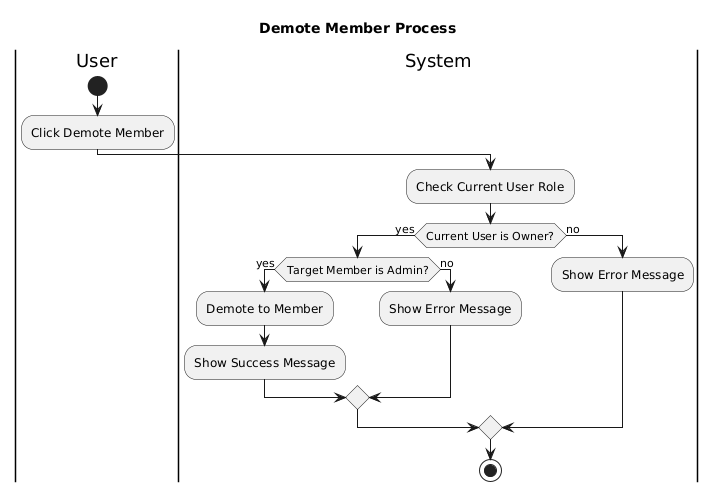
\includegraphics[width=0.8\textwidth]{assets/activity_diagrams/member_demote.png}
    \captionof{figure}{Activity Diagram Member Demote}
\end{center}
pada activity diagram diatas menjelaskan bahwa user dengan role owner bisa melakukan demosi admin menjadi member.

\begin{center}
    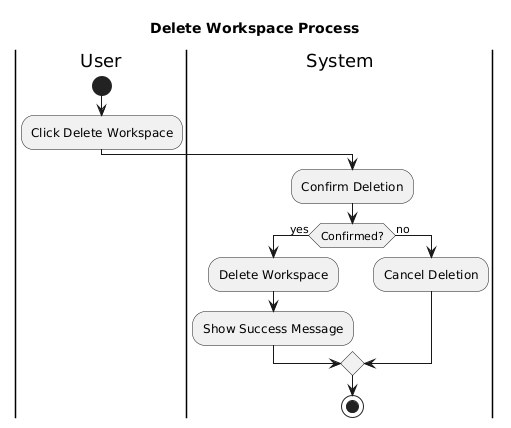
\includegraphics[width=0.5\textwidth]{assets/activity_diagrams/workspace_delete.png}
    \captionof{figure}{Activity Diagram Workspace Delete}
\end{center}
pada activity diagram diatas menjelaskan bahwa user dengan role owner bisa menghapus workspace yang sudah dibuat.

\subsubsection*{Task Management}
\begin{center}
    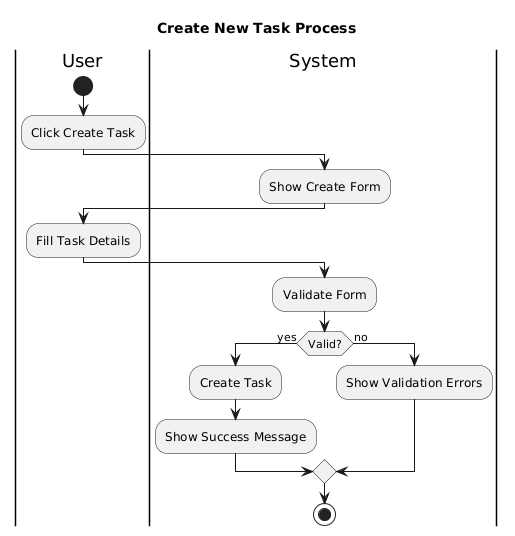
\includegraphics[width=0.5\textwidth]{assets/activity_diagrams/task_create.png}
    \captionof{figure}{Activity Diagram Task Create}
\end{center}
pada activity diagram diatas menjelaskan bahwa user dengan role admin dan owner bisa membuat task baru.

\begin{center}
    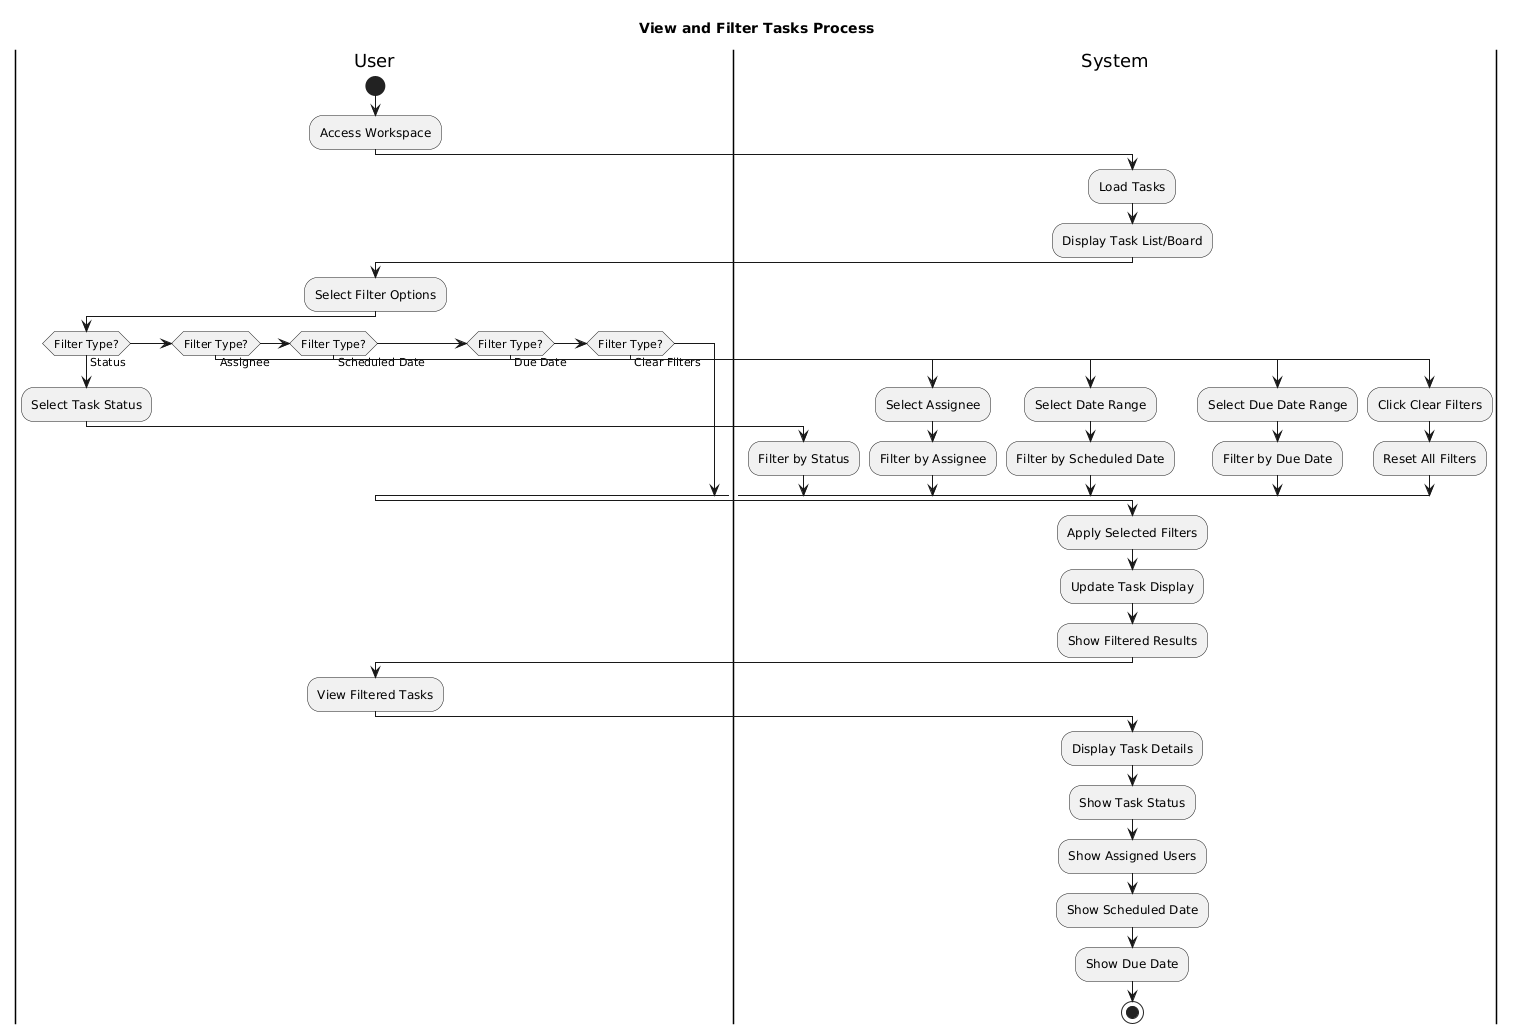
\includegraphics[width=1\textwidth]{assets/activity_diagrams/task_read.png}
    \captionof{figure}{Activity Diagram Task Read}
\end{center}
pada activity diagram diatas menjelaskan bahwa user dengan semua role bisa melihat task yang ada di dalam workspace tersebut.
disediakan juga fitur filter dan search untuk memudahkan user dalam mencari task yang dibutuhkan.

\begin{center}
    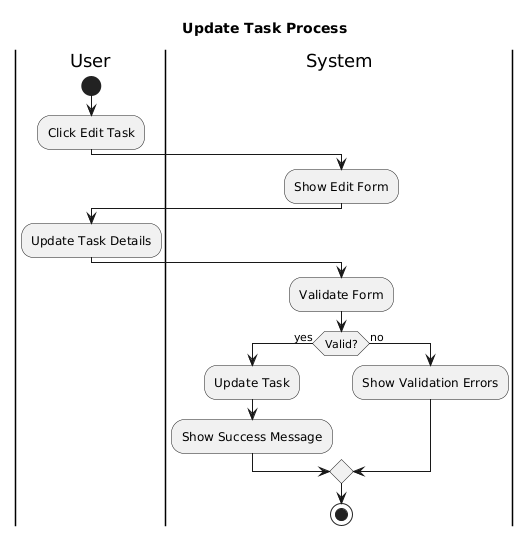
\includegraphics[width=0.5\textwidth]{assets/activity_diagrams/task_update.png}
    \captionof{figure}{Activity Diagram Task Update}
\end{center}
pada activity diagram diatas menjelaskan bahwa user dengan role admin dan owner bisa mengubah task yang sudah dibuat.

\begin{center}
    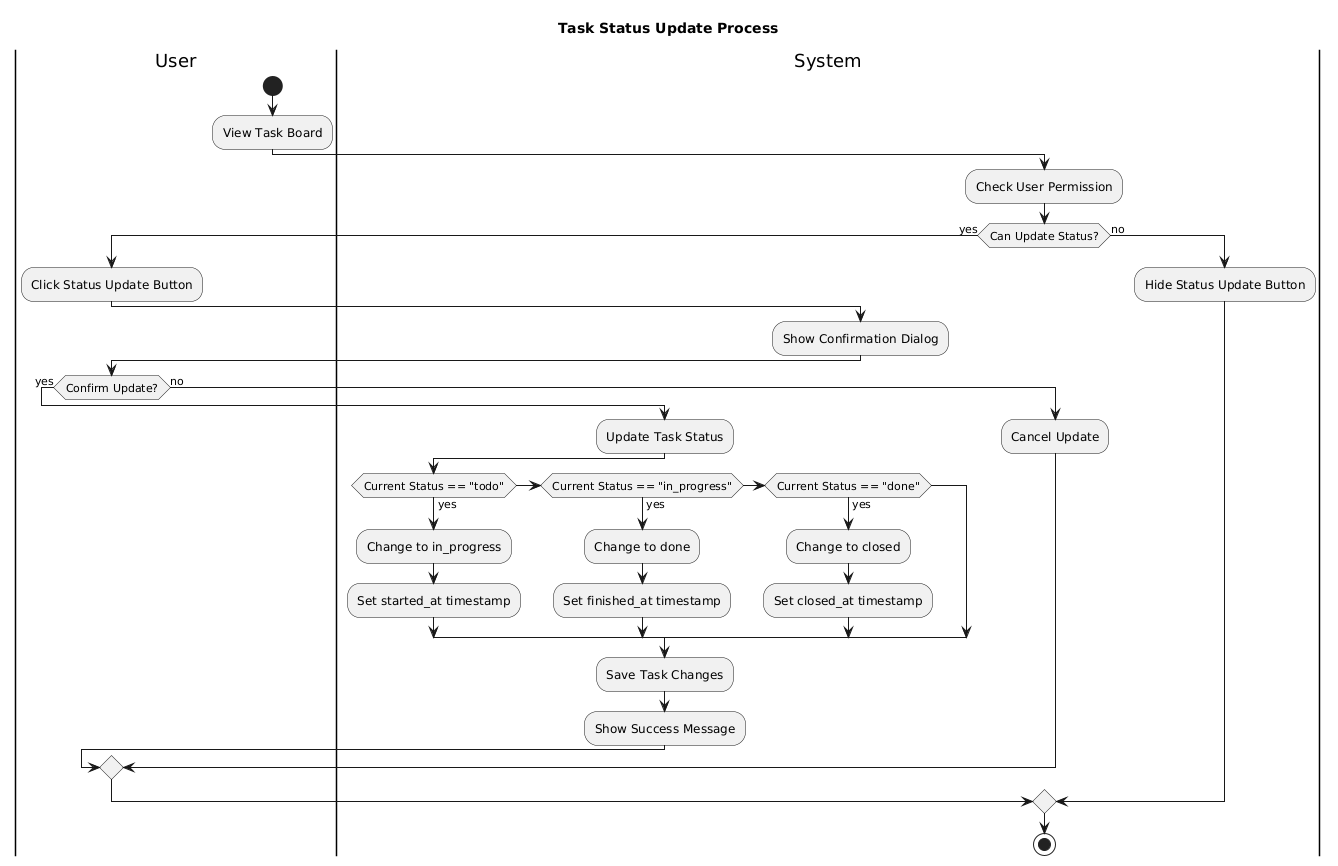
\includegraphics[width=0.8\textwidth]{assets/activity_diagrams/task_status_update.png}
    \captionof{figure}{Activity Diagram Task Status Update}
\end{center}
pada activity diagram diatas menjelaskan bahwa user dengan role admin dan owner bisa mengubah status task yang sudah dibuat.
untuk status task yang tersedia adalah todo, in progress, dan done. dari status todo, user bisa mengubah status menjadi in progress.
dari status in progress, user bisa mengubah status menjadi done. dan dari status done, user bisa mengubah status menjadi closed. 
closed adalah status task yang sudah selesai dan tidak aktif lagi (diarsipkan), task dengan status closed tidak akan muncul di board task.

\begin{center}
    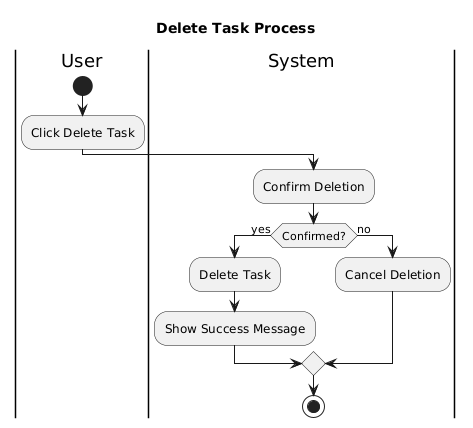
\includegraphics[width=0.5\textwidth]{assets/activity_diagrams/task_delete.png}
    \captionof{figure}{Activity Diagram Task Delete}
\end{center}
pada activity diagram diatas menjelaskan bahwa user dengan role admin dan owner bisa menghapus task yang sudah dibuat.

\begin{center}
    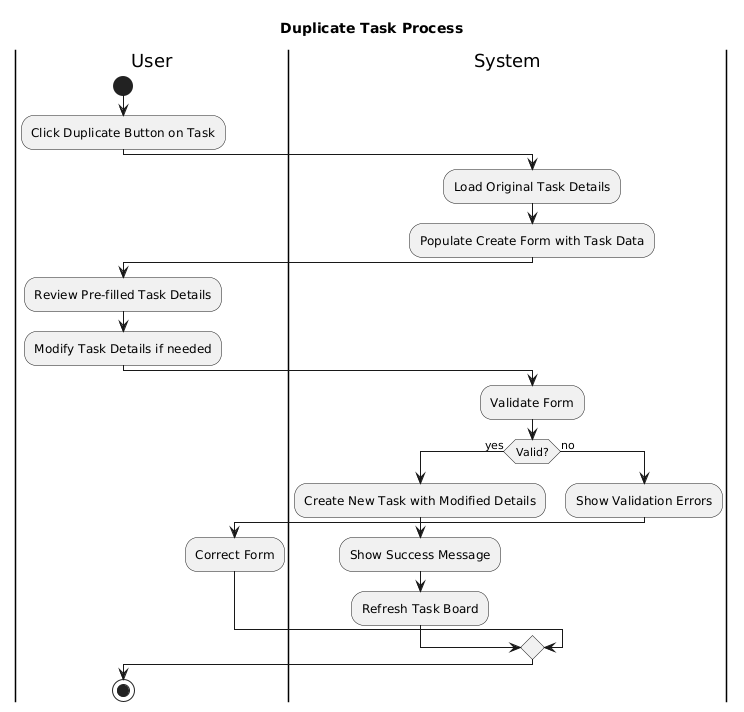
\includegraphics[width=0.5\textwidth]{assets/activity_diagrams/task_duplicate.png}
    \captionof{figure}{Activity Diagram Task Duplicate}
\end{center}
pada activity diagram diatas menjelaskan bahwa user dengan role admin dan owner bisa menyalin task yang sudah dibuat.
sehingga memudahkan user untuk membuat task baru yang mirip dengan task yang sudah ada.
\subsection*{3.8 ERD}
\begin{center}
  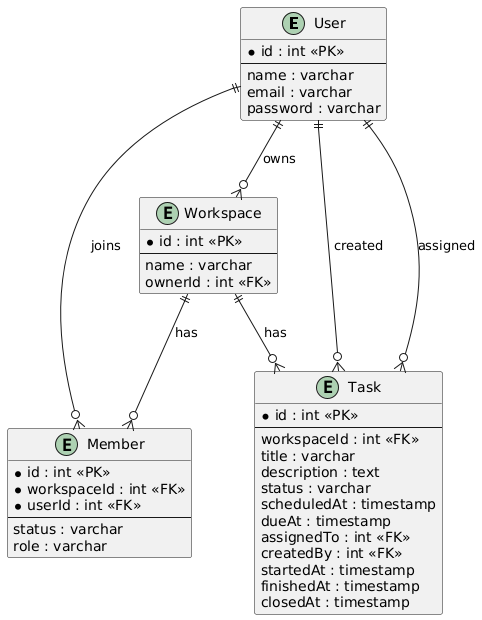
\includegraphics[width=0.8\textwidth]{assets/erd.png}
  \captionof{figure}{ERD}
\end{center}


\subsection*{3.9 Table Design}
Pada desain table berikut ini menjelaskan isi dari masing-masing table yang ada pada sistem. 
Pembuatan desain table ditujukan untuk mempermudah pembuatan database sistem, karena terdapat keterangan kolom primary key dan foreign key.

\subsubsection*{3.9.1	Tabel User}
\begin{center}
  \captionof{table}{Tabel 3.1 Struktur Tabel User}
  \begin{tabular}{|c|c|c|c|}
    \hline
    \textbf{Kolom} & \textbf{Tipe Data} & \textbf{Keterangan} \\
    \hline
    id & int & Primary Key, Id User \\
    name & varchar & Nama User \\
    email & varchar & Email User \\ 
    password & varchar & Password User \\
    created\_at & timestamp & Waktu pembuatan User \\
    updated\_at & timestamp & Waktu pembaruan User \\
    \hline
  \end{tabular}
\end{center}

Table user digunakan untuk menyimpan data user yang terdaftar pada sistem. primary key dari table ini adalah id.

\subsubsection*{3.9.2	Tabel Workspace}
\begin{center}
  \captionof{table}{Tabel 3.2 Struktur Tabel Workspace}
  \begin{tabular}{|c|c|c|c|}
    \hline
    \textbf{Kolom} & \textbf{Tipe Data} & \textbf{Keterangan} \\
    \hline
    id & int & Primary Key, Id Workspace \\
    name & varchar & Nama Workspace \\
    created\_by & int & Foreign Key, Id User \\
    created\_at & timestamp & Waktu pembuatan Workspace \\
    updated\_at & timestamp & Waktu pembaruan Workspace \\
    \hline
  \end{tabular}
\end{center}

Table workspace digunakan untuk menyimpan data workspace yang terdaftar pada sistem. primary key dari table ini adalah id.
table ini juga memiliki foreign key yaitu created\_by yang merupakan id dari user yang membuat workspace tersebut.

\subsubsection*{3.9.3	Tabel Member}
\begin{center}
  \captionof{table}{Tabel 3.3 Struktur Tabel Member}
  \begin{tabular}{|c|c|c|c|}
    \hline
    \textbf{Kolom} & \textbf{Tipe Data} & \textbf{Keterangan} \\
    \hline
    id & int & Primary Key, Id Member \\
    user\_id & int & Foreign Key, Id User \\
    workspace\_id & int & Foreign Key, Id Workspace \\
    created\_at & timestamp & Waktu pembuatan Member \\
    updated\_at & timestamp & Waktu pembaruan Member \\
    \hline
  \end{tabular}
\end{center}

Table member digunakan untuk menyimpan data member yang terdaftar pada workspace. primary key dari table ini adalah id.
table ini juga memiliki foreign key yaitu user\_id dan workspace\_id yang merupakan id dari user dan workspace yang terkait.
kolom role digunakan untuk menentukan role dari member pada workspace tersebut, role yang tersedia adalah member, admin, dan owner.

\subsubsection*{3.9.4	Tabel Task}
\begin{center}
  \captionof{table}{Tabel 3.4 Struktur Tabel Task}
  \begin{tabular}{|c|c|c|c|}
    \hline
    \textbf{Kolom} & \textbf{Tipe Data} & \textbf{Keterangan} \\
    \hline
    id & int & Primary Key, Id Task \\
    name & varchar & Nama Task \\
    description & text & Deskripsi Task \\
    status & varchar & Status Task \\
    created\_at & timestamp & Waktu pembuatan Task \\
    updated\_at & timestamp & Waktu pembaruan Task \\
    \hline
  \end{tabular}
\end{center}

Table task digunakan untuk menyimpan data task yang terdaftar pada workspace. primary key dari table ini adalah id.
table ini juga memiliki foreign key yaitu workspace\_id yang merupakan id dari workspace yang terkait.


